\section{Posterior}

\begin{frame}{Calculating Posterior for Year 1}

  \begin{itemize}
    \item Using Year 1 data, we treat the number of wins as following a Binomial distribution based on the total games played.
    \item This Binomial likelihood is combined with the Beta prior, resulting in a Beta distribution for our posterior.
    \item The posterior for Year 1 reflects our updated belief about the team’s win probability after observing Year 1 performance.
  \end{itemize}
  
\end{frame}

\begin{frame}{Updating the Prior Year-by-Year}

  \begin{itemize}
    \item For each subsequent year, we treat the posterior from the previous year as the new prior.
    \item This recursive process allows us to carry forward accumulated information, refining our estimate of the team’s win probability year after year.
  \end{itemize}
  
\end{frame}

\begin{frame}{Updating the Prior Year-by-Year}
    
\begin{figure}
  \centering
  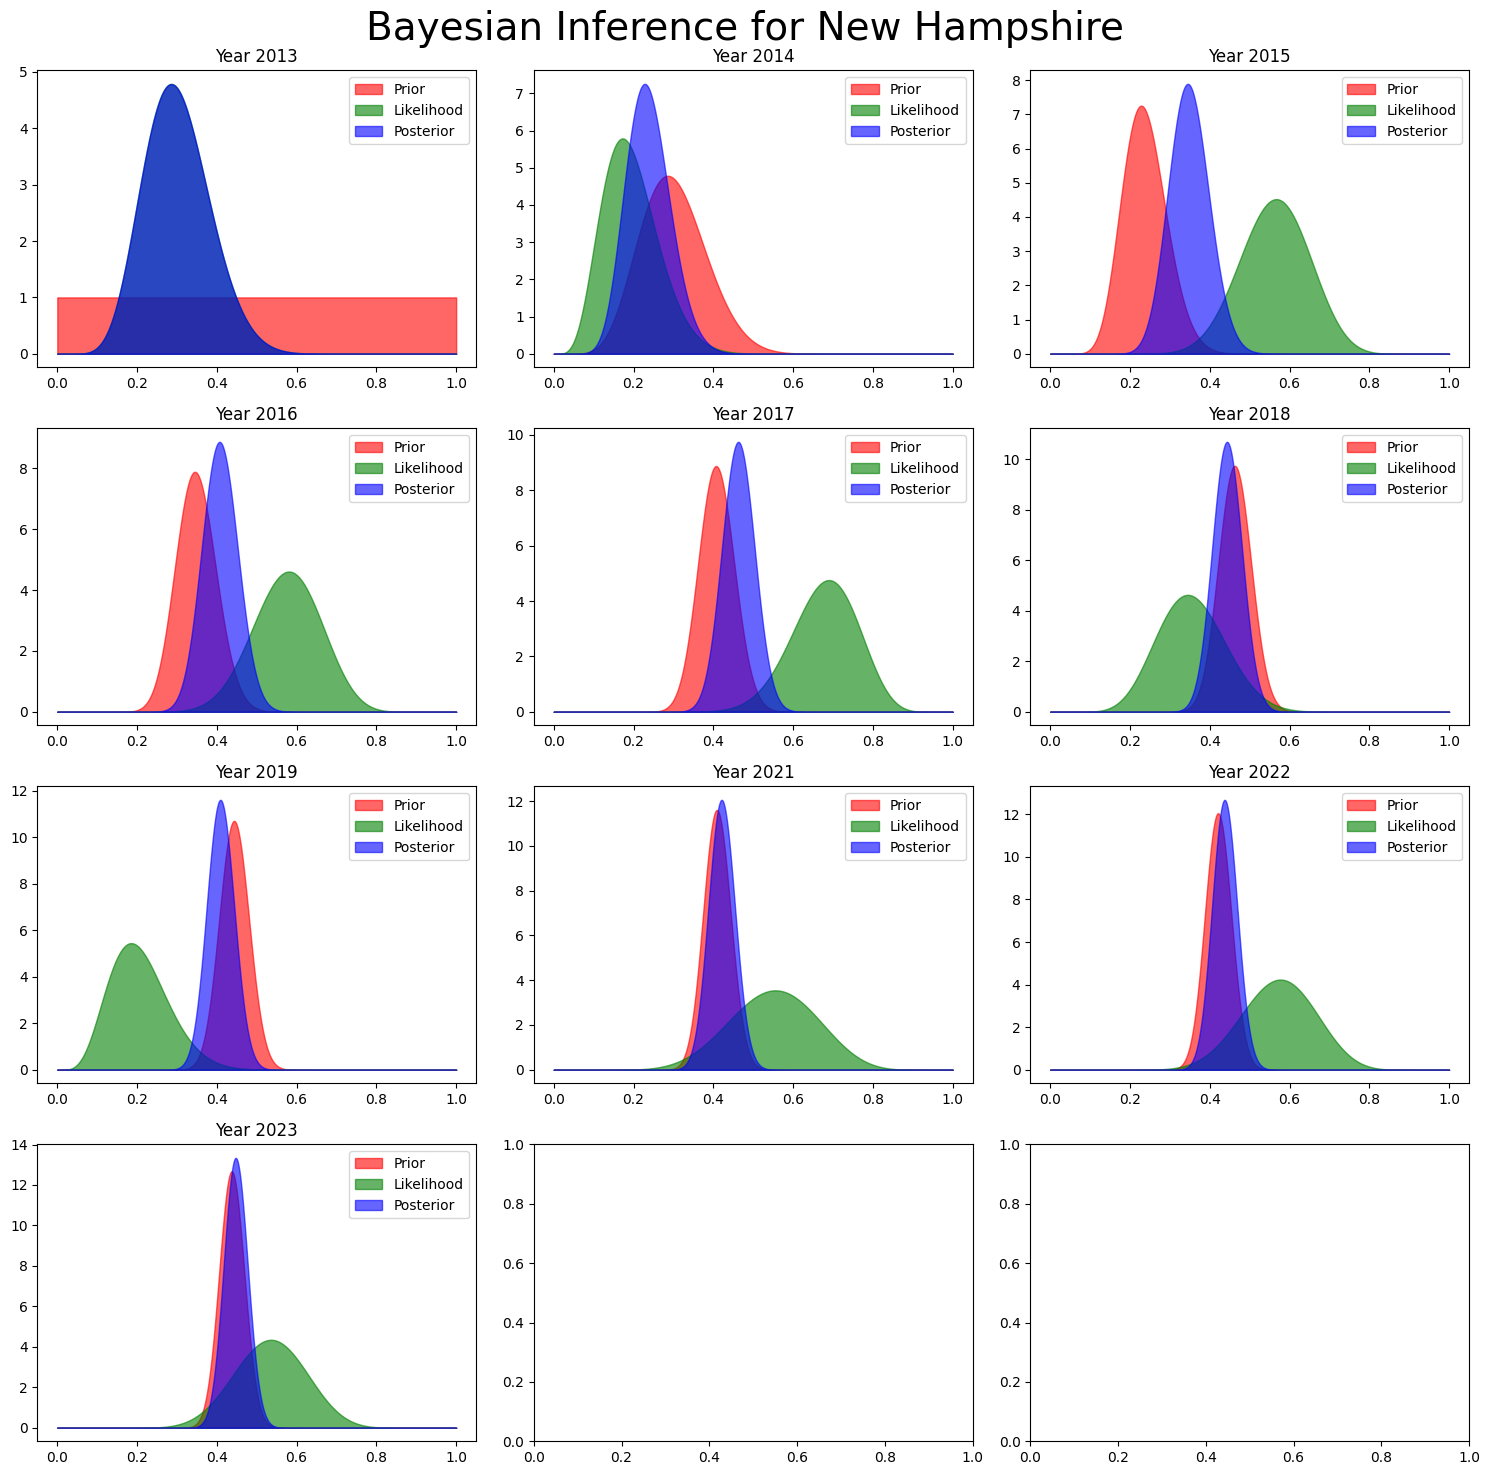
\includegraphics[width=.7\linewidth]{../Report/images/posterior-subplots.png}
  \caption{Prior, Likelihood and Posterior for each year}
\end{figure}

\end{frame}

\begin{frame}{Year-by-Year Posterior Distributions}

  \begin{itemize}
    \item Here, we visualize the evolution of the posterior distributions over each year.
    \item These distributions become more concentrated, indicating increased confidence as more data is incorporated over time.
  \end{itemize}

\begin{figure}
  \centering
  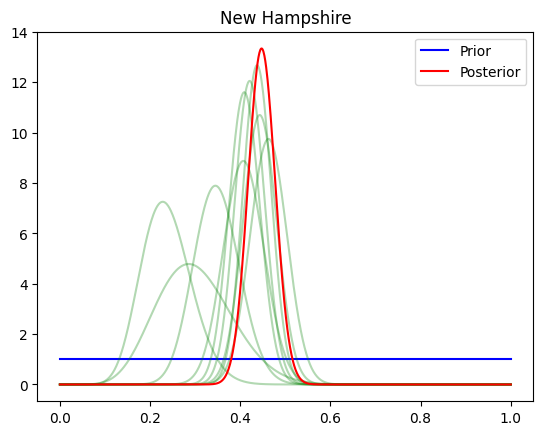
\includegraphics[width=.6\linewidth]{../Report/images/posterior-years.png}
  \caption{Posterior Distributions Over Years}
\end{figure}

  
\end{frame}
